%%%%%%%%%%%%%%%%%%%%%%%%%%%%%%%%%%%%%%%%%%%%%%%%%%%%%%%%%%%%%%%%%%%%%%%%%%%
%%
%%  LaTeX + CJK 模板,只针对 A4 纸的中文Paper。
%%
%%  Ver 1.02 By DeathKing @ <dk.hit.edu.cn>
%%  Ver 1.01 By rabbitbug @ www.ctex.org
%%  Ver 1.0 by oLo @ bbs.ustc.edu.cn
%%
%%  You can mofify it and distribute it freely:)
%%
%%%%%%%%%%%%%%%%%%%%%%%%%%%%%%%%%%%%%%%%%%%%%%%%%%%%%%%%%%%%%%%%%%%%%%%%%%%%

%%%%%%%%%%%%%%%%%%%%%%%%%%%%%%%%%%%%%%%%%%%%%%%%%%%%%%%%%%%%%%%%
%  文章模板:A4 纸,小五字,单列(可根据要求改双列 twocolumn)
%%%%%%%%%%%%%%%%%%%%%%%%%%%%%%%%%%%%%%%%%%%%%%%%%%%%%%%%%%%%%%%%
\documentclass[a4paper,11pt,onecolumn,twoside]{article}
%%%%%%%%%%%%%%%%%%%%%%%%%%%%%%%%%%%%%%%%%%%%%%%%%%%%%%%%%%%%%%%%
%  packages
%    这部分声明需要用到的包
%%%%%%%%%%%%%%%%%%%%%%%%%%%%%%%%%%%%%%%%%%%%%%%%%%%%%%%%%%%%%%%%
\usepackage{CJK}         % CJK 中文支持
\usepackage{fancyhdr}
\usepackage{amsmath,amsfonts,amssymb,graphicx}    % EPS 图片支持
\usepackage{subfigure}   % 使用子图形
\usepackage{indentfirst} % 中文段落首行缩进
\usepackage{bm}          % 公式中的粗体字符(用命令\boldsymbol)
\usepackage{multicol}    % 正文双栏
\usepackage{indentfirst} % 中文首段缩进
\usepackage{picins}      % 图片嵌入段落宏包 比如照片
\usepackage{abstract}    % 2栏文档,一栏摘要及关键字宏包
%%%%%%%%%%%%%%%%%%%%%%%%%%%%%%%%%%%%%%%%%%%%%%%%%%%%%%%%%%%%%%%%
%  lengths
%    下面的命令重定义页面边距,使其符合中文刊物习惯。
%%%%%%%%%%%%%%%%%%%%%%%%%%%%%%%%%%%%%%%%%%%%%%%%%%%%%%%%%%%%%%%%
\addtolength{\topmargin}{-54pt}
\setlength{\oddsidemargin}{-0.9cm}  % 3.17cm - 1 inch
\setlength{\evensidemargin}{\oddsidemargin}
\setlength{\textwidth}{17.00cm}
\setlength{\textheight}{24.00cm}    % 24.62
%%%%%%%%%%%%%%%%%%%%%%%%%%%%%%%%%%%%%%%%%%%%%%%%%%%%%%%%%%%%%%%%
%  定义标题格式,包括title,author,affiliation,email等。
%  在任何用到中文的地方,用\begin{CJK} ... \end{CJK}将其括起来。
%%%%%%%%%%%%%%%%%%%%%%%%%%%%%%%%%%%%%%%%%%%%%%%%%%%%%%%%%%%%%%%%

\renewcommand{\baselinestretch}{1.1} %定义行间距
\parindent 22pt %重新定义缩进长度

%%%%%%%%%%%%%%%%%%%%%%%%%%%%%%%%%%%%%%%%%%%%%%%%%%%%%%%%%%%%%%%%
% 标题,作者,通信地址定义
%%%%%%%%%%%%%%%%%%%%%%%%%%%%%%%%%%%%%%%%%%%%%%%%%%%%%%%%%%%%%%%%
\begin{CJK}{GBK}{song}
\title{\huge{王母娘娘寿筵上蟠桃生长过程\\
仿真与分析}\thanks{收稿日期:~XXXX$-$XX$-$XX. 基金项目:国家自然科学基金资助项目~(51685168)}}
\author{猴哥,八戒\\[2pt]
\normalsize
(新西方大学取经系,大唐省~长安市~123456) \\[2pt]}
\date{}  % 这一行用来去掉默认的日期显示
\end{CJK}

%%%%%%%%%%%%%%%%%%%%%%%%%%%%%%%%%%%%%%%%%%%%%%%%%%%%%%%%%%%%%%%%
% 首页页眉页脚定义
%%%%%%%%%%%%%%%%%%%%%%%%%%%%%%%%%%%%%%%%%%%%%%%%%%%%%%%%%%%%%%%%
\fancypagestyle{plain}{
\fancyhf{}
\lhead{第~XX~卷\quad 第~X~期\\
\scriptsize{XXXX~年~XX~月}}
\chead{\centering{西~~天~~取~~经~~记\\
\scriptsize{\textbf{The trip to get the Sutra}}}}
\rhead{Vol. XX, No. XX\\
\scriptsize{October, 2004}}
\lfoot{}
\cfoot{}
\rfoot{}}

%%%%%%%%%%%%%%%%%%%%%%%%%%%%%%%%%%%%%%%%%%%%%%%%%%%%%%%%%%%%%%%%
% 首页后根据奇偶页不同设置页眉页脚
% R,C,L分别代表左中右,O,E代表奇偶页
%%%%%%%%%%%%%%%%%%%%%%%%%%%%%%%%%%%%%%%%%%%%%%%%%%%%%%%%%%%%%%%%
\pagestyle{fancy}
\fancyhf{}
\fancyhead[RE]{第~XX~卷}
\fancyhead[CE]{西~~天~~取~~经~~记}
\fancyhead[LE,RO]{\thepage}
\fancyhead[CO]{猴~~哥等:王母娘娘寿筵上蟠桃生长过程仿真与分析}
\fancyhead[LO]{第~X~期}
\lfoot{}
\cfoot{}
\rfoot{}
%%%%%%%%%%%%%%%%%%%%%%%%%%%%%%%%%%%%%%%%%%%%%%%%%%%%%%%%%%%%%%%%
% 正文两栏环境不允许float环境,比如 figure, table。所以重新定义
% figure,使之可以浮动到你想要的位置。table也同样,把figure改为
% table就可以。
%%%%%%%%%%%%%%%%%%%%%%%%%%%%%%%%%%%%%%%%%%%%%%%%%%%%%%%%%%%%%%%%
\newenvironment{figurehere}
  {\def\@captype{figure}}
  {}
\makeatother


%%%%%%%%%%%%%%%%%%%%%%%%%%%%%%%%%%%%%%%%%%%%%%%%%%%%%%%%%%%%%%%%
%  文章正文
%%%%%%%%%%%%%%%%%%%%%%%%%%%%%%%%%%%%%%%%%%%%%%%%%%%%%%%%%%%%%%%%
\begin{document}
\begin{CJK*}{GBK}{song}
\CJKcaption{GB}
%%%%%%%%%%%%%%%%%%%%%%%%%%%%%%%%%%%%%%%%%%%%%%%%%%%%%%%%%%%%%%%%
%  自定义命令
%%%%%%%%%%%%%%%%%%%%%%%%%%%%%%%%%%%%%%%%%%%%%%%%%%%%%%%%%%%%%%%%
% 此行使文献引用以上标形式显示
\newcommand{\supercite}[1]{\textsuperscript{\cite{#1}}}
%%%%%%%%%%%%%%%%%%%%%%%%%%%%%%%%%%%%%%%%%%%%%%%%%%%%%%%%%%%%%%%%
%  显示title,并设页码为空(按杂志社要求)
%%%%%%%%%%%%%%%%%%%%%%%%%%%%%%%%%%%%%%%%%%%%%%%%%%%%%%%%%%%%%%%%
\maketitle

%%%%%%%%%%%%%%%%%%%%%%%%%%%%%%%%%%%%%%%%%%%%%%%%%%%%%%%%%%%%%%%%
%%%%%%%%%%%%%%%%%%%%%%%%%%%%%%%%%%%%%%%%%%%%%%%%%%%%%%%%%%%%%%%%
%  中文摘要
%  调整摘要、关键词,中图分类号的页边距
%  中英文同时调整
%%%%%%%%%%%%%%%%%%%%%%%%%%%%%%%%%%%%%%%%%%%%%%%%%%%%%%%%%%%%%%%%
\setlength{\oddsidemargin}{ 1cm}  % 3.17cm - 1 inch
\setlength{\evensidemargin}{\oddsidemargin}
\setlength{\textwidth}{13.50cm}
\vspace{-.8cm}
\begin{center}
\parbox{\textwidth}{
\CJKfamily{hei}摘~~~要\quad \CJKfamily{kai}~蟠桃真好吃,当时真是吃少了,现在需要研究研究,希望能给花果山的孩儿们栽上几棵,尝尝鲜。\\
\CJKfamily{hei}关键词\quad\CJKfamily{kai}蟠桃,王母娘娘,寿筵,天宫\\
\CJKfamily{hei}中图分类号\quad TG9527\qquad  \CJKfamily{hei}文献标识码\quad A}
\end{center}
%%%%%%%%%%%%%%%%%%%%%%%%%%%%%%%%%%%%%%%%%%%%%%%%%%%%%%%%%%%%%%%%
%  英文摘要
%%%%%%%%%%%%%%%%%%%%%%%%%%%%%%%%%%%%%%%%%%%%%%%%%%%%%%%%%%%%%%%%
\vspace{.1cm}
\begin{center}
\parbox{\textwidth}{
{\large{\textbf{Analysis and simulation of the peaches in the birthday party of lady Wang Mu}}}\\
\vspace{-0.5cm}
\begin{center}
\textbf{Hou Ge, Ba Jie}\\[2pt]
\small{\textit{(Dept. Qu Jing, New Western Univ., Changan Da Tang 123456, China)}}\\[2pt]
\end{center}
{\small{\textbf{Abstract}\quad The peaches in the birthday party of lady Wang Mu were so delicious that I want to dwell on the analysis and simulation on them. So that I can bring some of them to my kids in Hua Guo Shan.\\
\textbf{Key Words}\quad Peach, lady Wang Mu, birthday party, Heaven palace}}
}
\end{center}
%%%%%%%%%%%%%%%%%%%%%%%%%%%%%%%%%%%%%%%%%%%%%%%%%%%%%%%%%%%%%%%%
%  文章编号(左上角)
%%%%%%%%%%%%%%%%%%%%%%%%%%%%%%%%%%%%%%%%%%%%%%%%%%%%%%%%%%%%%%%%
\begin{minipage}[c]{10cm}
\vspace{-35.5cm}
文章编号~~~~1005$-$0388(2004)05$-$0505$-$04
\end{minipage}
%%%%%%%%%%%%%%%%%%%%%%%%%%%%%%%%%%%%%%%%%%%%%%%%%%%%%%%%%%%%%%%%
%  正文由此开始-------------------------
%%%%%%%%%%%%%%%%%%%%%%%%%%%%%%%%%%%%%%%%%%%%%%%%%%%%%%%%%%%%%%%%
%%%%%%%%%%%%%%%%%%%%%%%%%%%%%%%%%%%%%%%%%%%%%%%%%%%%%%%%%%%%%%%%
%  恢复正文页边距
%%%%%%%%%%%%%%%%%%%%%%%%%%%%%%%%%%%%%%%%%%%%%%%%%%%%%%%%%%%%%%%%
\setlength{\oddsidemargin}{-.5cm}  % 3.17cm - 1 inch
\setlength{\evensidemargin}{\oddsidemargin}
\setlength{\textwidth}{17.00cm}
\CJKfamily{song}
%%%%%%%%%%%%%%%%%%%%%%%%%%%%%%%%%%%%%%%%%%%%%%%%%%%%%%%%%%%%%%%%
%  分栏开始
\begin{multicols}{2}
%%%%%%%%%%%%%%%%%%%%%%%%%%%%%%%%%%%%%%%%%%%%%%%%%%%%%%%%%%%%%%%%
\section{引言}
%%%%%%%%%%%%%%%%%%%%%%%%%%%%%%%%%%%%%%%%%%%%%%%%%%%%%%%%%%%%%%%%
%  调整section名称与正文之间的距离
%%%%%%%%%%%%%%%%%%%%%%%%%%%%%%%%%%%%%%%%%%%%%%%%%%%%%%%%%%%%%%%%
文献\supercite{Wu,Xuan}中提到:一朝,王母娘娘设宴,大开宝阁,瑶池中做“蟠桃胜会”,即着那红衣仙女、素衣仙女、青衣仙女
、皂衣仙女、紫衣仙女、黄衣仙女、绿衣仙女,各顶花篮,去蟠桃园摘桃建会。七衣仙女直至园门首,
只见蟠桃园土地、力士同齐天府二司仙吏,都在那里把门。仙女近前道:“我等奉王母懿旨,到此携桃
设宴。”土地道:“仙娥且住。今岁不比往年了,玉帝点差齐天大圣在此督理,须是报大圣得知,方敢
开园。”仙女道:“大圣何在?”土地道:“大圣在园内,因困倦,自家在亭子上睡哩。”仙女道:“
\begin{figure*}
\centering
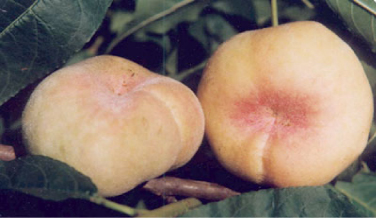
\includegraphics[width=12cm]{Pantao.jpg}
\caption{王母娘娘寿筵上的蟠桃}\label{fig2}
\end{figure*}
既如此,寻他去来,不可延误。”土地即与同进。寻至花亭不见,只有衣冠在亭,不知何往。四下里都
没寻处。原来大圣耍了一会,吃了几个桃子,变做二寸长的个人儿,在那大树梢头浓叶之下睡着了。七衣
仙女道:“我等奉旨前来,寻不见大圣,怎敢空回?”旁有仙吏道:“仙娥既奉旨来,不必迟疑。我大圣
闲游惯了,想是出园会友去了。汝等且去摘桃,我们替你回话便是。”那仙女依言,入树林之下摘桃。先
在前树摘了二篮,又在中树摘了三篮;到后树上摘取,只见那树上花果稀疏,止有几个毛蒂青皮的。原来
熟的都是猴王吃了。七仙女张望东西,只见南枝上止有一个半红半白的桃子。青衣女用手扯下枝来,红衣
女摘了,却将枝子望上一放。原来那大圣变化了,正睡在此枝,被他惊醒。大圣即现本相,耳朵内掣出金
箍棒,幌一幌,碗来粗细,咄的一声道:“你是那方怪物,敢大胆偷摘我桃!”慌得那七仙女一齐跪下道
:“大圣息怒。我等不是妖怪,乃王母娘娘差来的七衣仙女,摘取仙桃,大开宝阁,做‘蟠桃胜会’。适
至此间,先见了本园土地等神,寻大圣不见。我等恐迟了王母懿旨,是以等不得大圣,故先在此摘桃,万
望恕罪。”大圣闻言,回嗔作喜道:“仙娥请起。王母开阁设宴,请的是谁?”仙女道:“上会自有旧规。
请的是西天佛老、菩萨、罗汉,南方南极观音,东方崇恩圣帝,十洲三岛仙翁,北方北极玄灵,中央黄极黄
角大仙,这个是五方五老。还有五斗星君,上八洞三清、四帝、太乙天仙等众,中八洞玉皇、九垒、海岳神
仙,下八洞幽冥教主、注世地仙。各宫各殿大小尊神,俱一齐赴蟠桃嘉会。”大圣笑道:“可请我么?”仙
女说:“不曾听得说。”大圣道:“我乃齐天大圣,就请我老孙做个尊席,有何不可?”仙女道:“此是上
会会规,今会不知如何。”大圣道:“此言也是,难怪汝等。你且立下,待老孙先去打听个消息,看可请老孙不请。”
好大圣,捻着诀,念声咒语,对众仙女道:“住!住!住!”这原来是个定身法,把那七衣仙女一
个个睖睖睁睁,白着眼,都站在桃树之下。大圣纵朵祥云,跳出园内,竟奔瑶池路上而去。\\
\indent 名称赤脚大罗仙,特赴蟠桃添寿节。那赤脚大仙觌面撞见大圣,大圣低头定计,赚哄真仙,他要暗去赴会,
却问:“老道何往?”大仙道:“蒙王母见招,去赴蟠桃嘉会。”大圣道:“老道不知。玉帝因老孙筋斗云疾,
着老孙五路邀请列位,先至通明殿下演礼,后方去赴宴。”大仙是个光明正大之人,就以他的诳语作真。道:“
常年就在瑶池演礼谢恩,如何先去通明殿演礼,方去瑶池赴会?”无奈,只得拨转祥云,径往通明殿去了。\\
\indent 大圣驾着云,念声咒语,摇身一变,就变做赤脚大仙模样,前奔瑶池。不多时,直至宝阁,按住云头,轻轻
移步,走入里面。只见那里:
琼香缭绕,瑞霭缤纷,瑶台铺彩结,宝阁散氤氲。凤翥鸾腾形缥缈,金花玉萼影浮沉。上排着九凤丹霞扆,
八宝紫霓墩。五彩描金桌,千花碧玉盆。桌上有龙肝和凤髓,熊掌与猩唇。珍馐百味般般美,异果嘉肴色色新。
\section{结论}
\begin{figurehere}
\centering
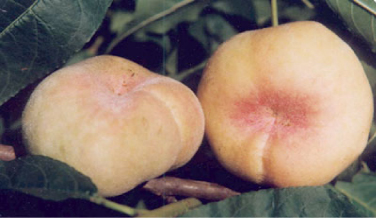
\includegraphics[width=6cm]{Pantao.jpg}
\caption{王母娘娘寿筵上的蟠桃}\label{fig2}
\end{figurehere}
%%%%%%%%%%%%%%%%%%%%%%%%%%%%%%%%%%%%%%%%%%%%%%%%%%%%%%%%%%%%%%%%
%  参考文献
%%%%%%%%%%%%%%%%%%%%%%%%%%%%%%%%%%%%%%%%%%%%%%%%%%%%%%%%%%%%%%%%
\small
\begin{thebibliography}{99}
\setlength{\parskip}{0pt}  %段落之间的竖直距离
\bibitem{Wu}吴承恩. 西游记~[M], 明14XX年.
\bibitem{Xuan} 玄奘. 大唐西域记学报~[J], 唐~6XX~年, 1(2): 23-55.

\end{thebibliography}
%%%%%%%%%%%%%%%%%%%%%%%%%%%%%%%%%%%%%%%%%%%%%%%%%%%%%%%%%%%%%%%%
% 作者简历,段落插入图片用picins宏包和\parpic命令
%%%%%%%%%%%%%%%%%%%%%%%%%%%%%%%%%%%%%%%%%%%%%%%%%%%%%%%%%%%%%%%%
\normalsize
\parpic{%
\includegraphics[width=3.0cm]%
{Hou.jpg}}
\indent 猴~~哥~~($xxx-$),男,江苏花果山人,法号行者,是唐僧的大徒弟,会七十二变、腾云驾雾。
一双火眼金睛,能看穿妖魔鬼怪伪装的伎俩;一个筋斗能翻十万八千里;使用的兵器如意金箍棒,能大能小,
随心变化,小到绣花针,大到顶天立地。他占花果山为王,自称齐天大圣,搅乱王母娘娘的蟠桃胜会,
偷吃太上老君的长生不老金丹,打败天宫十万天兵天将,又自不量力地与如来佛祖斗法,被压在五行山下五百多年。
后来经观世音菩萨点化,保护唐僧西天取经,三打白骨精,收服红孩儿,熄灭火焰山,一路上降魔斗妖,
历经九九八十一难,取回真经终成正果。他嫉恶如仇,不怕困难,坚韧不拔,英勇无畏,取经后被封为斗战胜佛。\\
\indent 八~~戒~~($xxx-$),男,天宫人,法号悟能,是唐僧的二徒弟,原来是玉皇大帝的天蓬元帅,
因调戏嫦娥被逐出天界,到人间投胎,却又错投猪胎,嘴脸与猪相似。他会变身术,能腾云驾雾,
使用的兵器是九齿钉钯。唐僧西去取经路过云栈洞,猪八戒被孙悟空收服,八戒从此成为孙悟空的好帮手,
一同保护唐僧西天取经。八戒性格温和,憨厚单纯,力气大,但又好吃懒做,爱占小便宜,贪图女色,
经常被妖怪的美色所迷,难分敌我。他对师兄的话言听计从,对师父忠心耿耿,为唐僧西天取经立下汗马功劳,
是个被人们喜爱同情的喜剧人物。
%%%%%%%%%%%%%%%%%%%%%%%%%%%%%%%%%%%%%%%%%%%%%%%%%%%%%%%%%%%%%%%%
%  分栏结束
%%%%%%%%%%%%%%%%%%%%%%%%%%%%%%%%%%%%%%%%%%%%%%%%%%%%%%%%%%%%%%%%
\end{multicols}
%%%%%%%%%%%%%%%%%%%%%%%%%%%%%%%%%%%%%%%%%%%%%%%%%%%%%%%%%%%%%%%%
%  文章结束
%%%%%%%%%%%%%%%%%%%%%%%%%%%%%%%%%%%%%%%%%%%%%%%%%%%%%%%%%%%%%%%%
\clearpage
\end{CJK*}
\end{document}